\section{Vision 3D}
    Pour ce problème de docking, nous avons besoin de fixer un repère associé à chaque robot. Ce repère va permettre de déterminer la position de ceux-ci dans le repère monde et cela va s’avérer être nécessaire afin d’accoupler un robot sur un autre.

    Il va donc falloir être en mesure de connaître à chaque instant la position et l’orientation de chaque robot. Il existe plusieurs solutions pour cela. D’abord il est possible d’utiliser un système de positionnement GNSS. Ils présentent l’avantage d’être relativement bas coûts et assez précis. Cependant, il est connu que la couverture GNSS doit être bonne pour utiliser ce genre de capteurs. De plus, le positionnement avec des systèmes classiques n’est précis qu’à quelques mètres près. Il est donc peu probable que ce capteur soit satisfaisant lors de la phase d’approche finale. On ne peut pas se permettre d’accoupler deux robots alors que leur position n’est pas connue avec une bonne précision. Enfin ce capteur seul n’est pas en mesure de donner une information sur l’orientation d’un robot.

    Une autre solution qui semble intéressante est d’utiliser le docking visuel. L’idée est d’utiliser des caméras qui sont des capteurs aujourd’hui peu coûteux et qui fournissent beaucoup d’informations sur la scène. Le docking visuel est donc basé sur l’utilisation de ces capteurs afin d’acquérir la position des robots dans le repère monde. Pour cela, deux techniques peuvent être mises en œuvre : une technique en caméra fixe dans le repère monde et une technique avec des caméras embarquées sur les robots.

    Ces solutions à base de caméra pour réaliser du docking sont déjà utilisées dans l’industrie. La société Forssea Robotics a développé et commercialisé une caméra capable de réaliser cette tâche, appelée Navcam~\cite{forssea}. Elle permet de localiser des marqueurs dans une scène et de renvoyer des repères associés à ces marqueurs. On est donc capable d’avoir la position et aussi l’orientation des robots si on dispose ces marqueurs sur nos robots. Ces caméras possèdent l’avantage d’être complètement étanches et elles peuvent résister à des pressions importantes. Cela leur permet d’être embarquées sur des robots sous-marins pouvant aller jusqu’à 3000 mètres de profondeur (ROVs ou AUV). La \textsc{Figure}~\ref{fig:navcam} nous montre cette caméra.

    \begin{figure}[!htb]
        \centering
        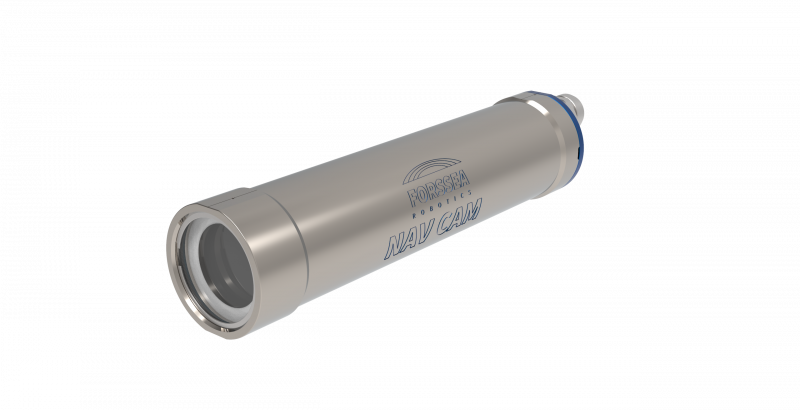
\includegraphics[width=0.5\textwidth]{./vision_3d/navcam.png}
        \caption{Navcam commercialisée par Forssea Robotics}
        \label{fig:navcam}
    \end{figure}

    Cette caméra se base sur l’utilisation d’ArUco qui est une bibliothèque minimale permettant de mettre en œuvre de la réalité augmentée. Le principe est exactement de pouvoir repérer la position et l’orientation d’un marqueur dans la scène à l’aide d’une caméra. Cependant, ils ont modifié les marqueurs en y ajoutant des points noirs sur le pourtour afin d’avoir une plus grande précision sur les attitudes fournies, et de la robustesse face à la turbidité par exemple qui est souvent présente dans le milieu sous-marin.

    \begin{figure}[!htb]
        \centering
        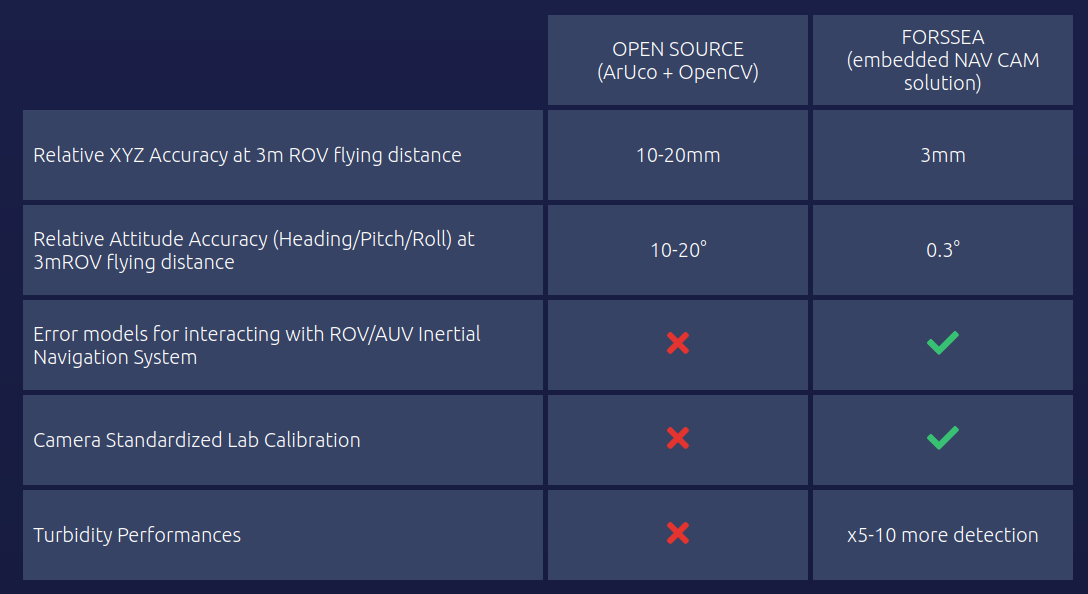
\includegraphics[width=0.6\textwidth]{./vision_3d/tableau.png}
        \caption{Comparaison des solutions de positionnement visuel proposées par la librairie Aruco et Forssea Robotics, \textit{source : \textit{https://opencv.org/} ; \url{https://forssea-robotics.fr/}}}
        \label{fig:tableau}
    \end{figure}

    L’avantage de cette caméra est qu’elle fournit une solution très simple de positionnement visuel de marqueurs dans la scène, compacte et industrialisée. Il est donc possible de mettre en œuvre ce capteur dans une application robotique, et les repères associés à chaque marqueur sont directement accessibles via une API. Cela est possible grâce au fait que la caméra est calibrée en usine et qu’elle embarque une carte de traitement électronique, la Nvidia Jetson Nano, qui permet d’effectuer le traitement numérique d’image permettant la détermination des différents repères. Des algorithmes d’intelligence artificielle vont aussi être implémentés afin de robustifier les prédictions dans le cas où le marqueur ne serait pas visible sur toutes les images.

    \begin{figure}[!htb]
        \centering
        \begin{subfigure}[b]{0.3\textwidth}
            \centering
            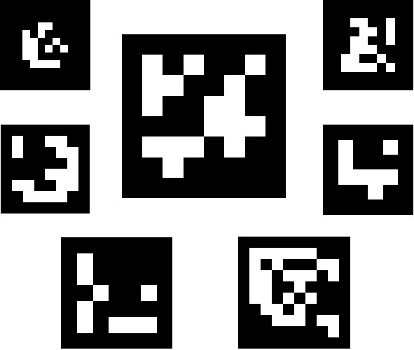
\includegraphics[width=\textwidth]{./vision_3d/marker.jpg}
            \caption{Marqueurs ArUco}
            \label{fig:marker}
        \end{subfigure}
        \hfill
        \begin{subfigure}[b]{0.6\textwidth}
            \centering
            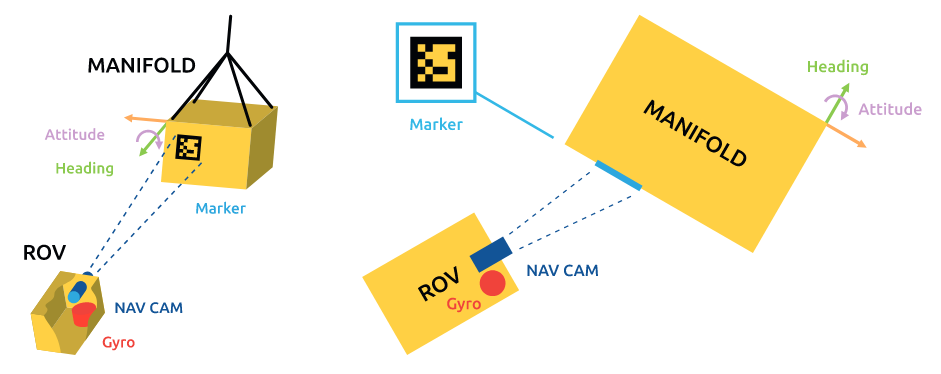
\includegraphics[width=\textwidth]{./vision_3d/manifold.png}
            \caption{Positionnement visuel}
            \label{fig:manifold}
        \end{subfigure}
        \caption{Exemple d'environnement mettant en jeu du docking visuel, \textit{source : \url{https://forssea-robotics.fr/}}}
        \label{fig:environnement}
    \end{figure}

    La solution avec une caméra fixe dans le repère monde est intéressante, car elle va permettre de directement donner la position des deux robots qui vont devoir s’accoupler dans le repère monde. On a donc accès aux repères associés à chaque robot et le but va être de déterminer la loi de commande permettant de faire converger leur position. Cependant elle pose deux problèmes, d’abord, il va falloir avoir disposé la caméra à un endroit fixe de la scène. C’est une contrainte forte. Il sera difficile voir impossible dans certaines situations de l’installer. Par exemple, dans le cas d’inspection de parcs éoliens offshores, il est impensable de devoir positionner un pylône pour soutenir une caméra ayant une vue globale sur la scène. Deuxièmement, il va falloir déterminer les paramètres extrinsèques de cette caméra, c'est-à-dire sa position et son orientation par rapport au repère monde. Cette étape indispensable va permettre de fournir les positions absolues des marqueurs dans la scène, chose qui semble indispensable à notre application. Cela constitue en soit une limite importante à cette solution.
    
    Quant à la solution avec des caméras embarquées, elle semble résoudre le problème d’une installation et de calibration de la caméra au préalable. De plus, une caméra embarquée sur un robot est directement connectée aux systèmes de navigation des robots et alimentée par celui-ci. Il faut néanmoins être en mesure de la transporter à bord d’un robot. Pour notre application de docking, nous avons donc deux possibilités : embarquer la caméra sur le drone, ou sur la plateforme au sol. 

    L’embarquement de la caméra sur l’UGV peut poser des problèmes de reflets sur l’image captée par la caméra, car elle peut dans certains cas être éblouie par la lumière du soleil, et donc ne plus être en mesure de détecter le marqueur disposé sur l’UAV. Cette solution présentait tout de même l’avantage de pouvoir transporter des batteries plus grosses, permettant d’avoir une plus grande autonomie, pour le système, mais aussi d’être plus stable, parce que le mouvement d’un UGV est bien plus stable que celui d’un UAV.

    L’embarquement de la caméra sur l’UAV est une solution qui pallie les éventuels problèmes de reflets sur l’image captée, mais il faut être en mesure de transporter la caméra sans déstabiliser le drone, mais aussi être en mesure de l’alimenter. C’est quelque chose qui n’est pas facilement faisable avec la Navcam de Forssea Robotics, car elle pèse plus de 3 kg et a besoin d’être alimentée par une batterie fournissant 24 volts. Trouver un drone permettant de transporter une telle charge utile n’est pas aisé, mais le piloter en toute sécurité et avoir les permissions l’est encore moins. C’est pourquoi, bien que la solution industrielle semble tout à fait intéressante, elle n’en reste pas moins inadaptée à notre application. Il faut en outre prévoir un ordinateur embarqué qui possède un port ethernet afin d'y interfacer la Navcam.

    Une idée qui permet de résoudre notre problème est d’utiliser la caméra embarquée sur la plupart des drones commerciaux et la librairie open-source d’ArUco~\cite{kurosu2018human, campilho2018image}. Étant dans un environnement moins contraint que pour des drones sous-marins, dont la visibilité n’est pas toujours bonne, cette solution semble suffire à détecter des marqueurs classiques de la bibliothèque ArUco et à obtenir leur position dans le repère de l’UAV. Au passage, il n’y a désormais besoin que d’avoir un marqueur sur l’UGV, et nous obtenons une position relative d’un robot par rapport à un autre ; nous nous sommes affranchis du repère monde, et l’implémentation devrait fonctionner peu importe l’endroit dans le monde.

    L’idée est donc dans un premier temps de calibrer la caméra afin de disposer de ses paramètres intrinsèques~\cite{corke2017robotics}. Ces paramètres permettent de déterminer à la fois les paramètres intrinsèques linéaires, c’est à dire la distance focale, les paramètres d'échelle et les paramètres de centrage de l’axe optique, mais aussi les paramètres intrinsèques non-linéaires de distorsion liés aux imperfections de l’objectif. La librairie OpenCV\footnote{\url{https://opencv.org}} propose une procédure de calibration basée sur l’algorithme de Levenberg-Marquardt\footnote{\url{https://docs.opencv.org/master/d3/d6d/classcv_1_1LMSolver.html}}~\cite{kurosu2018human, corke2017robotics}. Cela permet de pouvoir calculer les coordonnées d’un point dans le repère caméra en fonction des coordonnées du pixel capté dans l’image.

    Pour calibrer la caméra, il suffit de capturer un certain nombre d'images d’une mire de calibration qui ici est un échiquier, dont on connaît précisément les dimensions~\cite{corke2017robotics}. Un nœud ROS est développé sur la base de la librairie OpenCV et permet de réaliser cette action avec une interface graphique, comme le montre la \textsc{Figure}~\ref{fig:checkerboard}. On obtient en sortie un fichier avec tous les coefficients intrinsèques de la caméra qui nous servira pour les prochaines implémentations.

    \begin{figure}[!htb]
        \centering
        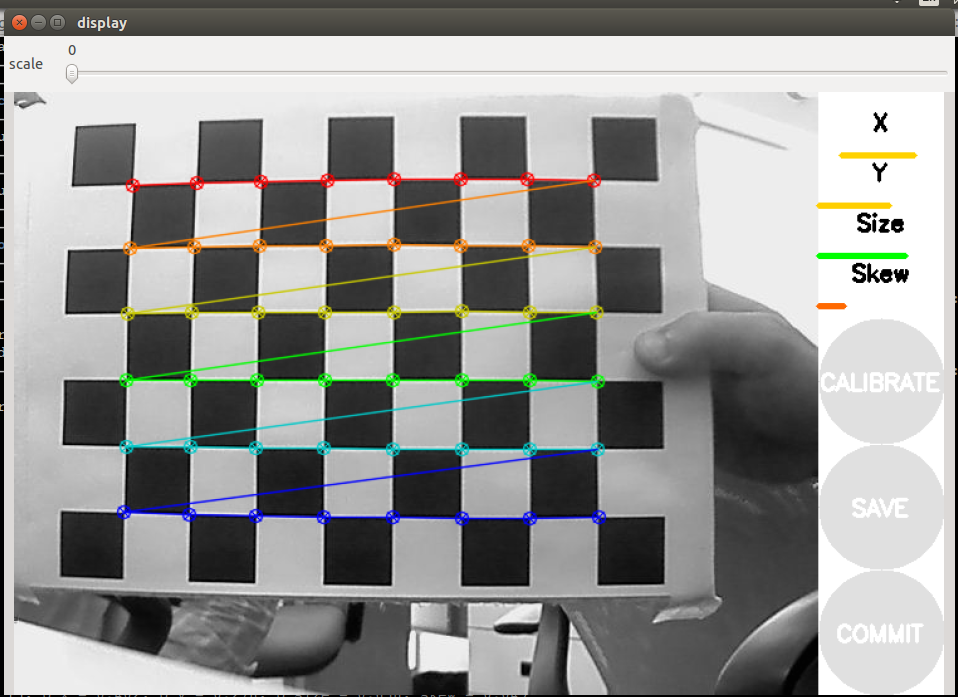
\includegraphics[width=0.6\textwidth]{./vision_3d/checkerboard.png}
        \caption{Calibration de la caméra du drone à l'aide d'un échiquier, \textit{source : \url{https://opencv.org}}}
        \label{fig:checkerboard}
    \end{figure}

    Ensuite, un nœud ROS est disponible afin de réaliser le traitement d’image et de détecter les marqueurs dans la scène. C'est le nœud \textit{aruco\_detect}\footnote{\url{http://wiki.ros.org/aruco_detect}}. Il fournit en sortie, si la caméra est calibrée, les coordonnées des repères associés aux marqueurs et nous permet donc de déterminer la position de l’UGV dans le repère de l’UAV, comme le montre la \textsc{Figure}~\ref{fig:detection}.

    \begin{figure}[!htb]
        \centering
        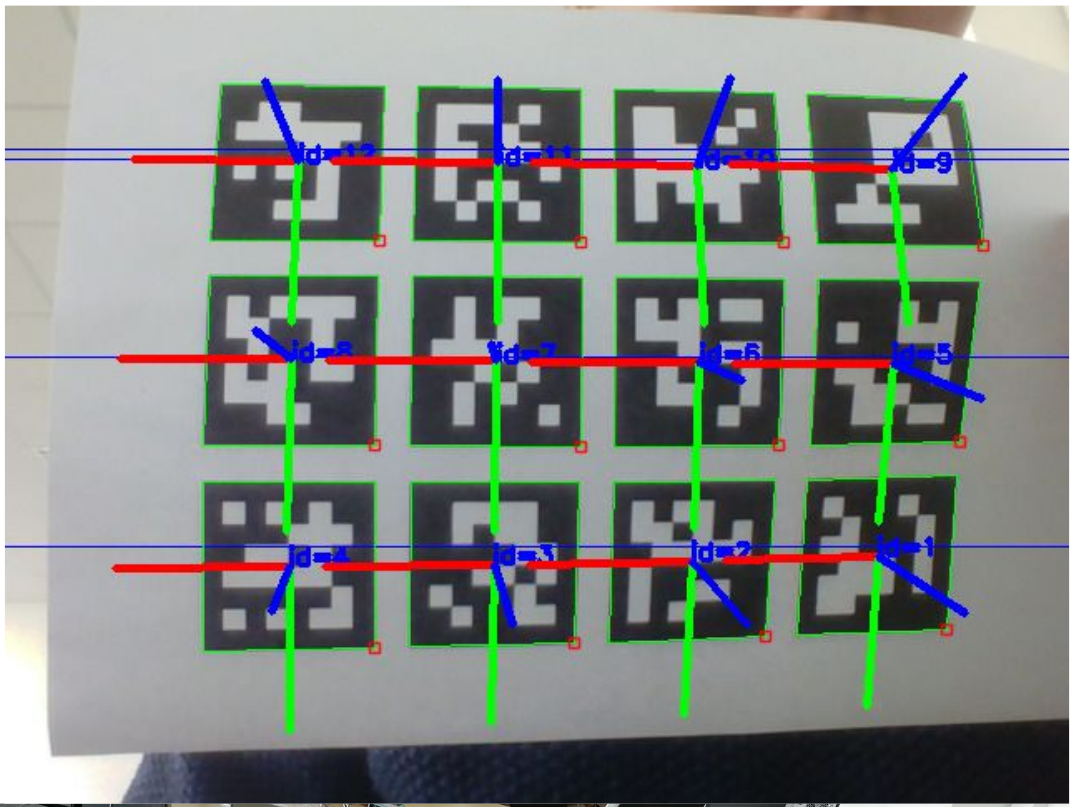
\includegraphics[width=0.6\textwidth]{./vision_3d/detection_markers.png}
        \caption{Detection de marqueurs ArUco à l'aide du n\oe ud ROS \textit{aruco\_detect}}
        \label{fig:detection}
    \end{figure}

    Ainsi nous sommes en mesure de déterminer la position de l’UGV dans le repère de l’UAV, ce qui ne semble pas usuel à première vue, car il aurait été plus intuitif de récupérer les repères associés aux robots dans le repère monde, mais comme nous avons pu le constater ces solutions ne sont pas envisageable pour notre application.

    Le placement des marqueurs Arco sur la plateforme arrière de l’UGV permettant la réception de l’UAV est important. En effet, le drone devra être capable de détecter les marqueurs de loin afin de pouvoir connaître sa position relative à la plateforme au sol. Mais il faut aussi qu’il puisse avoir une bonne estimation de sa position tout au long de sa descente, même lorsque certains marqueurs sortent du champ de vision de la caméra ou bien deviennent trop gros pour être complètement vus. C’est pourquoi il est nécessaire de disposer plusieurs marqueurs de tailles différentes sur la plateforme comme on a pu le constater dans la plupart des applications, comme par exemple pour le challenge DJI SDK challenge de 2016~\footnote{\url{https://www.youtube.com/watch?v=DIRkzH3cTAM}}. La \textsc{Figure}~\ref{fig:dji} présente la disposition des marqueurs ArUco extraite de la vidéo du challenge.

    \begin{figure}[!htb]
        \centering
        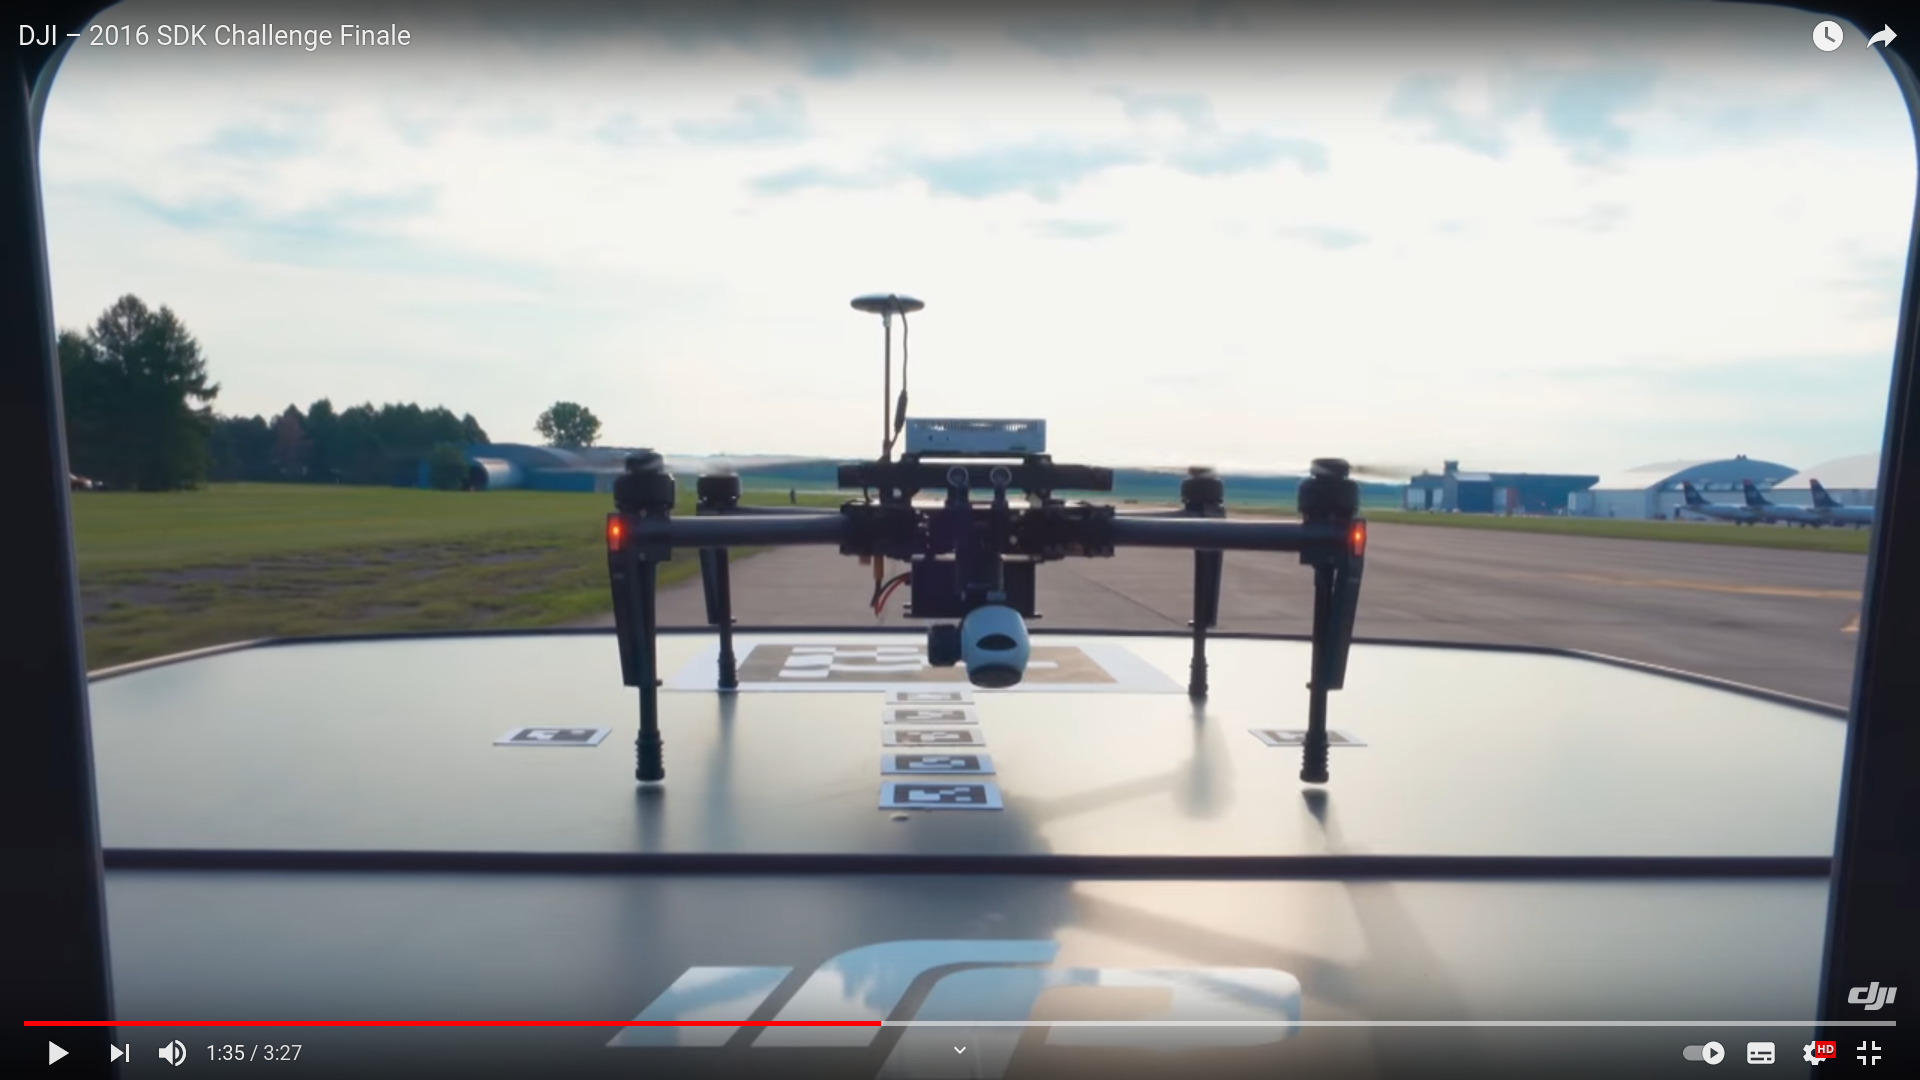
\includegraphics[width=0.5\textwidth]{./vision_3d/dji.png}
        \caption{DJI SDK Challenge 2016}
        \label{fig:dji}
    \end{figure}

    Nous avons donc décidé de disposer un marqueur de grande taille permettant une détection de loin de la plateforme d’accueil par la caméra de l’UAV, mais aussi des marqueurs de plus petite taille permettant d’être détectés lors de la phase finale du docking, qui permettent d’avoir plus de précision notamment sur les angles qui sont détectés avec peu de précision. La \textsc{Figure}~\ref{fig:marqueurs_ugv} présente la disposition des marqueurs sur la plateforme de l'UGV.
    
    \begin{figure}[!htb]
        \centering
        \begin{subfigure}[b]{0.35\textwidth}
            \centering
            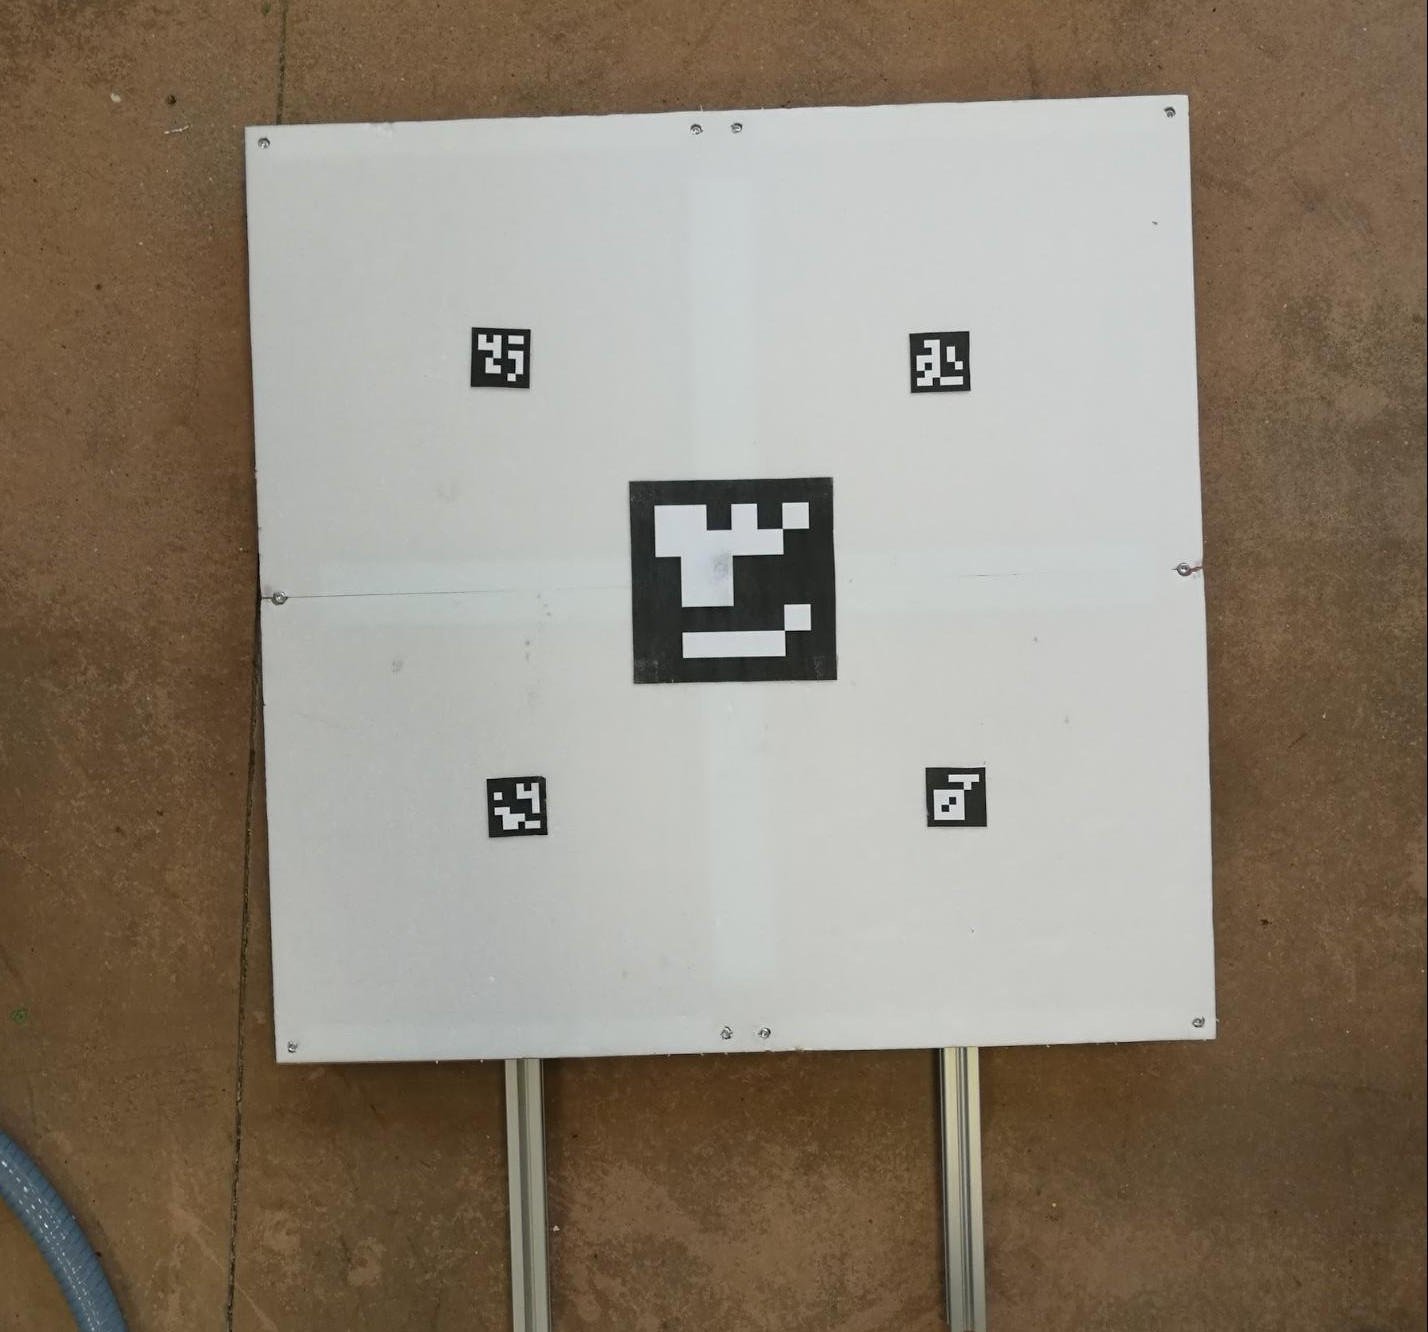
\includegraphics[width=\textwidth]{./vision_3d/plateau.jpg}
            \caption{Plateforme d'accueuil}
            \label{fig:plateforme}
        \end{subfigure}
        \hfill
        \begin{subfigure}[b]{0.55\textwidth}
            \centering
            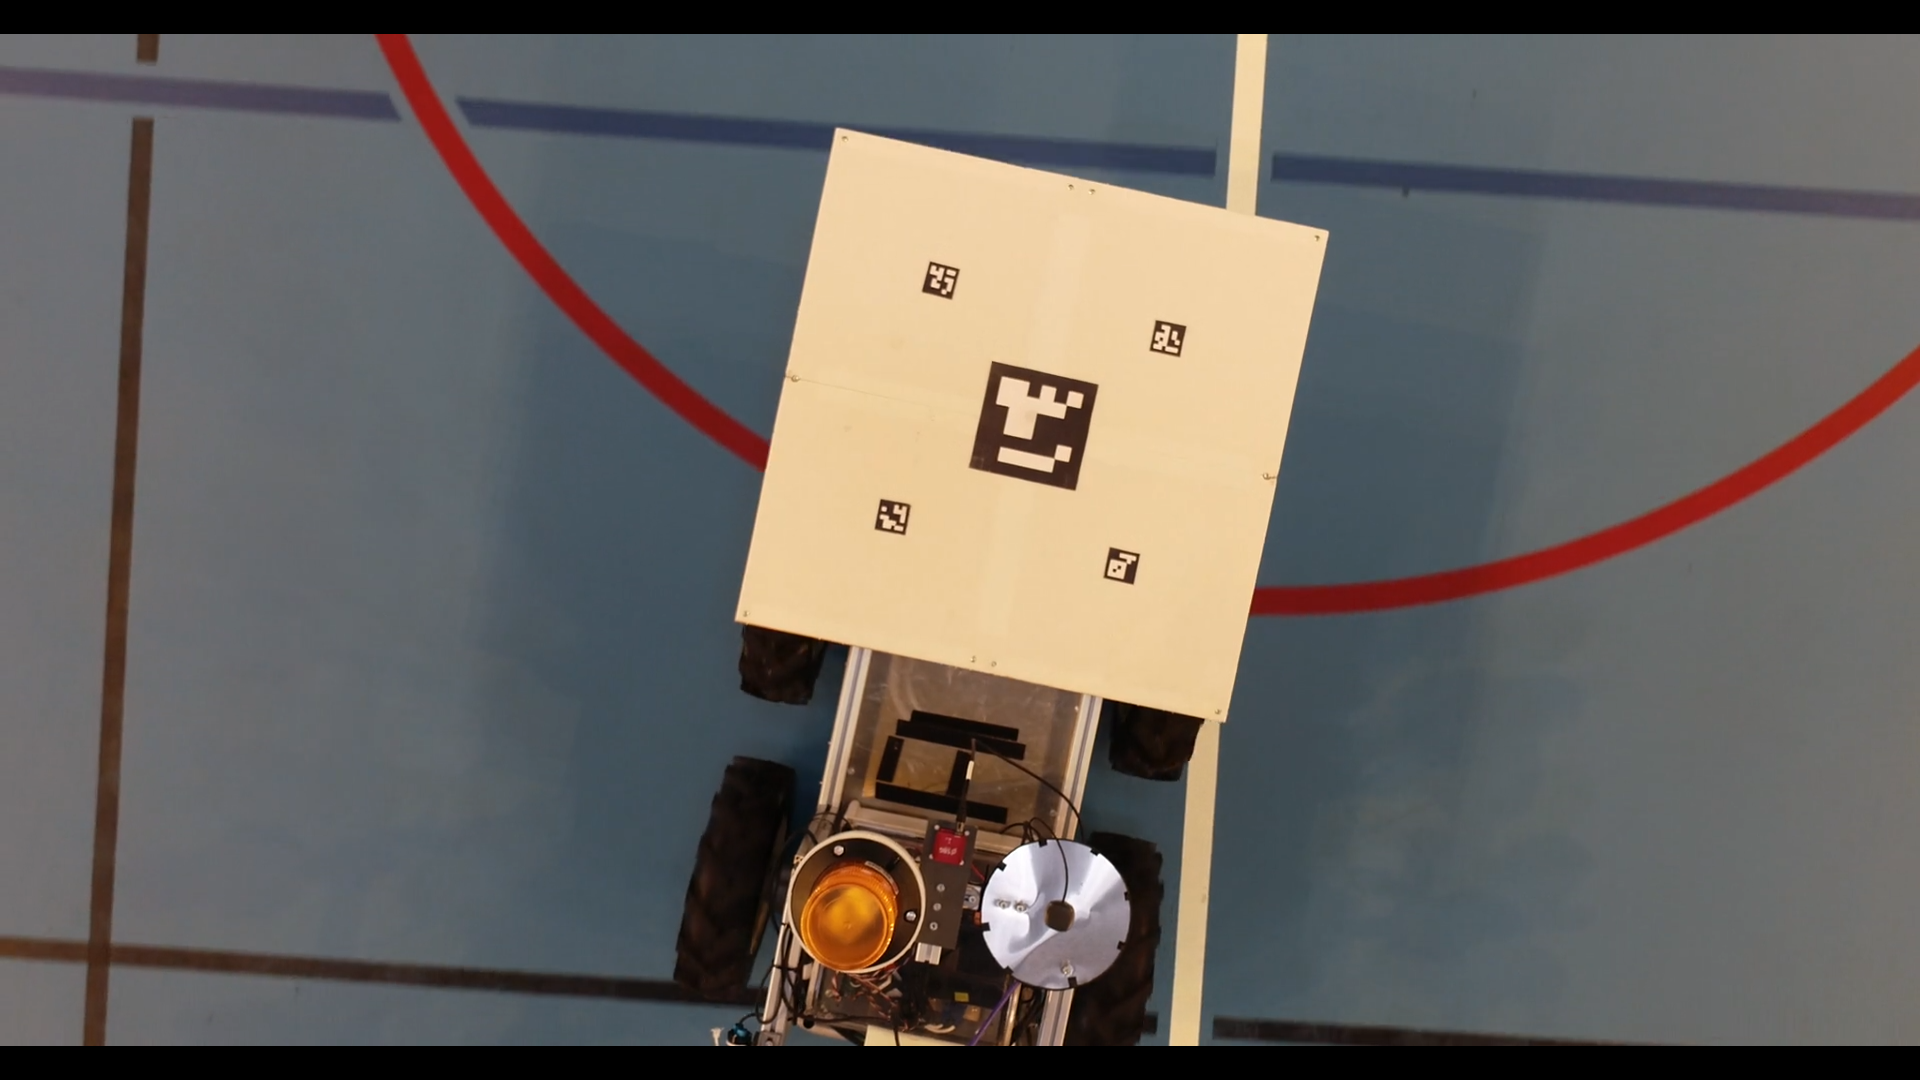
\includegraphics[width=\textwidth]{./vision_3d/ugv.png}
            \caption{Plateforme et marqueurs perçus par la caméra du drone}
            \label{fig:ugv}
        \end{subfigure}
        \caption{Disposition des marqueurs sur l'UGV}
        \label{fig:marqueurs_ugv}
    \end{figure}

    Lors d’essais, nous avons pu réaliser par exemple un atterrissage de l’UAV sur l’UGV puis son redécollage. On a obtenu la position et l’orientation du drone dans le repère de l’UGV uniquement grâce à la détection de marqueurs avec la caméra embarquée sur le drone. Les \textsc{Figures}~\ref{fig:results} présentent ces résultats. La position est très précise alors que l’orientation du drone est assez mal captée. Une technique de filtration a donc été nécessaire pour obtenir des informations pertinentes sur l’attitude du drone. Il y a d’abord une étape de suppression des outliers par médiane glissante et suppression des points trop éloignés. Ensuite on applique un filtre de butterworth permettant de supprimer le bruit présent sur les signaux. Avec cette méthode on estime avoir une précision de positionnement de l'ordre de $10\ cm$ et de l'ordre de $10\ deg$. Cette précision est estimable en supposant que le bruit de mesure est centré autour de la vraie valeur et que le bruit mesurable est un bruit blanc gaussien. Nous n'avions en outre aucun moyen de mesurer cette précision, dans la mesure où nous nous trouvions en intérieur et le GNSS n'était pas disponible.

    \begin{figure}[!htb]
        \centering
        \begin{subfigure}[b]{0.45\textwidth}
            \centering
            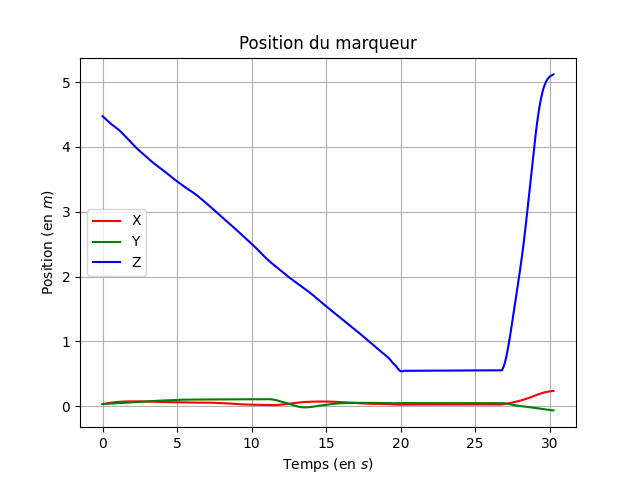
\includegraphics[width=\textwidth]{./vision_3d/positions.png}
            \caption{Positions estimées de l'UGV dans le repère de l'UAV}
            \label{fig:plateforme}
        \end{subfigure}
        \hfill
        \begin{subfigure}[b]{0.45\textwidth}
            \centering
            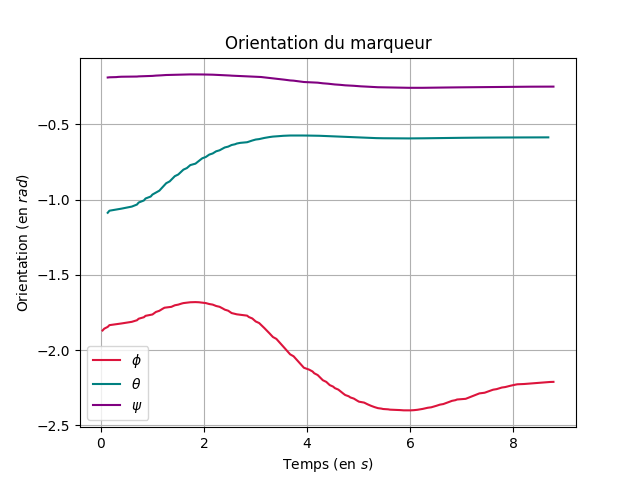
\includegraphics[width=\textwidth]{./vision_3d/angles.png}
            \caption{Angles d'Euler estimés de l'UGV dans le repère de l'UAV}
            \label{fig:ugv}
        \end{subfigure}
        \caption{Positionnement du repère de l'UGV dans le repère de l'UAV}
        \label{fig:results}
    \end{figure}
